
\section{Introduction}
% see you tomorrow

Recent years have witnessed rapid progress in text-conditioned 3D human motion generation, driven by advances in diffusion~\cite{tevet2022human} and transformer-based modeling~\cite{guo2022generating,guo2024momask}.
These models can synthesize diverse and realistic motion sequences from natural language prompts, enabling applications in character animation, AR/VR, embodied agents, and human--computer interaction.

A key catalyst behind recent progress is the emergence of large-scale motion--language datasets.
Early benchmarks such as KIT-ML~\cite{Plappert2016} and HumanML3D~\cite{guo2022generating} established the standard text-to-motion setting with paired clip-level captions and standardized evaluation.
However, these captions are typically short and describe an entire motion clip coarsely, limiting fine-grained controllability and semantic grounding. More recent datasets~\cite{han2024amd,wang2024scaling,punnakkal2021babel,xudense,li2026frankenmotion} broaden the supervision spectrum with richer long-form descriptions, hierarchical text annotations, frame-level action labels, and temporally localized captions. Together, these developments highlight a growing demand for \emph{fine-grained temporal correspondence} between motion and language, especially for long-form narratives and multi-action descriptions.
\begin{figure*}[h]
    \centering
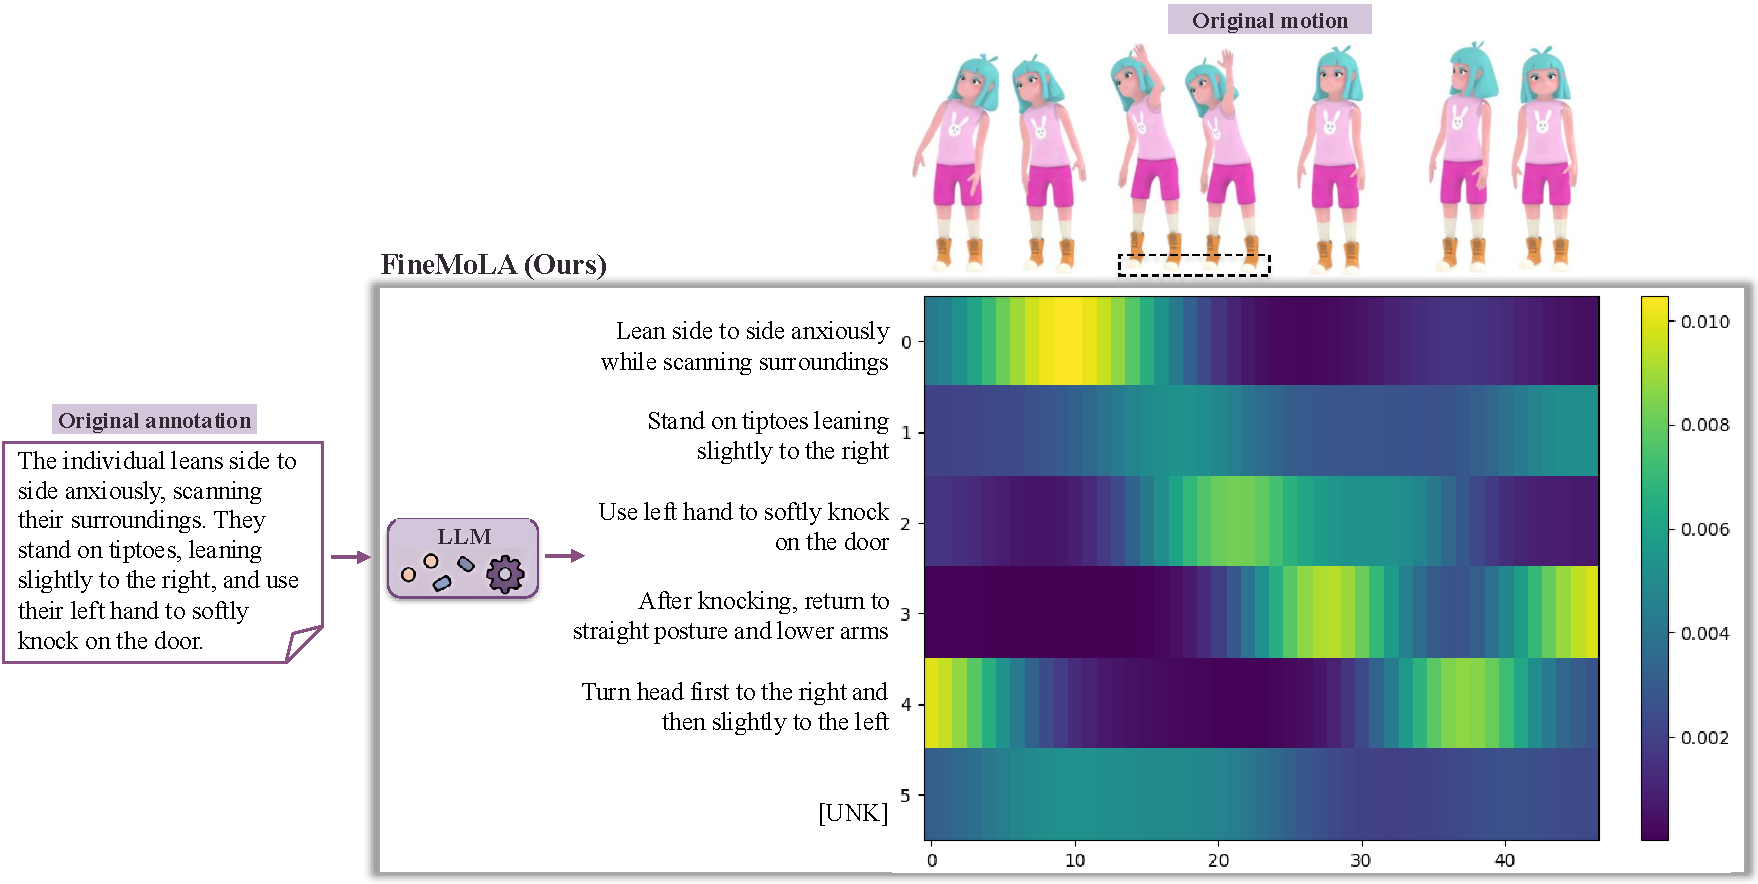
\includegraphics[width=\linewidth]{author-kit-CVPR2026-v1-latex-/figs/teaser.pdf}
    \caption{While the SnapMoGen dataset provides human motions with long-form text annotations, \ours finds the fine-grained alignment matrix between motion frames and LLM-detected action-bearing phrases in the text without manual labeling. Our method includes an \texttt{[UNK]} token to absorb frames that are not explicitly described by any specific phrase. The dashed black box highlights that the character does stand on tiptoes in those frames.}
    \label{fig:teaser}
\end{figure*}


Among existing datasets, SnapMoGen~\cite{guo2025snapmogen} stands out for its high-quality motion–language supervision. Its motions are collected using professional mocap suits, and its annotations are primarily written by human annotators. In contrast to earlier datasets that rely on short action labels or simple captions, SnapMoGen provides long-form descriptions that often cover multiple actions and transitions within a single motion clip. Such expressive supervision offers a strong foundation for studying fine-grained motion–text correspondence. However, the annotations remain at the clip level, without explicit frame-to-token alignment between motion and language. Learning such fine-grained correspondence could benefit motion understanding tasks such as temporal localization and dense motion captioning, and provide stronger supervision for fine-grained text-to-motion generation with temporal structure~\cite{wu2025mg,xudense,zhang2023finemogen}. At the same time, obtaining dense open-vocabulary alignment at scale remains challenging due to the inherently many-to-many relationships between words and motion over time.

As illustrated in \cref{fig:teaser}, we aim to recover fine-grained frame--phrase correspondence from long-form clip-level annotations without requiring manual temporal labels. To bridge this gap, we propose a semi-supervised framework that formulates frame--token correspondence as an optimal transport (OT) problem \cite{cuturi2013sinkhorn,peyre2019computational}.
Optimal transport naturally models many-to-many soft alignments under global marginal constraints, making it well-suited for motion-text grounding. To enable efficient and differentiable learning, we adopt entropic regularization and solve the resulting transport plan using Sinkhorn iterations \cite{cuturi2013sinkhorn}.
This formulation aligns with a broader trend in multimodal learning where fine-grained token-level alignment objectives improve cross-modal consistency and robustness \cite{yao2021filip,zhang2025pre,linmulti}.
Leveraging abundant clip-level supervision in SnapMoGen, our method produces pseudo frame-level alignments that support temporally grounded motion--language modeling.

To summarize, our contributions are as follows:
\begin{itemize}
\item We introduce \ours, a semi-supervised framework that learns fine-grained motion--language correspondence from clip-level annotations. By formulating frame-to-token alignments as an optimal transport problem, our method learns fine-grained correspondences for long-form textual descriptions, enabling dense motion--text grounding without requiring manual frame-level labels.
\item Experiments on the SnapMoGen dataset demonstrate that the learned alignments provide stronger motion--text grounding than baselines.
\end{itemize}

